\documentclass[a4,12pt]{scrartcl}

%Basic 
\usepackage[utf8]{inputenc}
\usepackage[ngerman]{babel}
\usepackage[T1]{fontenc}
%Schrift 
%\usepackage{fontspec} 
%\setmainfont{Arial} 
%Zeilenabstand
\usepackage{setspace}
\setstretch {1.3}
\usepackage{float}
\usepackage[bottom = 3.50cm]{geometry}

%Titel Seite
\usepackage{titling} %Wird benötigt damit \maketitle die Variabeln title, author und date nicht überschreibt
\title{Test Cases}
\subtitle{Projekt: software name}
\author{David Meister \and Andreas Stalder}		
 %mit /and können Personen hinzugefügt werden
\date{\today}


%Kopf, Fusszeile
\usepackage{fancyhdr}
\pagestyle{fancy}
\lhead{}
\chead{}
\rhead{software name}
\lfoot{\thetitle \: v1.0 }
\cfoot{\today }
\rfoot{Seite \thepage}
\renewcommand{\headrulewidth}{0.4pt}

%Bilder
\usepackage{graphicx}

%Zeichnen
\usepackage{tikz}

%Tabellen
\usepackage{booktabs}
\usepackage{longtable}

%Codesnippets
\usepackage{listings}
\lstset{language=java,basicstyle=\footnotesize,frame=single} %backgroundcolor=\color{lightgray}

%Querformat für eine Seite
\usepackage{lscape}
\usepackage{rotating}
\usepackage{pdflscape}

%URL 
\usepackage[colorlinks=true, linkcolor=blue, urlcolor=blue, citecolor=blue]{hyperref}
\urlstyle{same} 


%Loremimpsum
\usepackage{lipsum}



\begin{document}

%\clearpage\maketitle
\begin{titlepage}
	\centering
	\vspace{5cm}
	\begin{center}
%	\includegraphics[width=0.50\textwidth]{}
	\end{center}
	{\huge\bfseries software name\par}
	\vspace{8cm}
	\raggedright
	{\bfseries HSR Studienarbeit Network Unit Testing\par}
	{\huge\bfseries Network testing\par}
	\vspace{1cm}
	{\theauthor \par}
	{\today\par}

\end{titlepage}

\section{Änderungsgeschichte}

\begin{table}[htb]
\centering
    \begin{tabular}{@{} l l l l@{}}\toprule    
    {Datum} & {Version} & {Änderung} & {Autor}\\ \midrule
    27.09.16 & 1.0 & Erstellung erster Version & dm/as\\ \addlinespace
    \end{tabular}
\caption{\textbf{Änderungsgeschichte}}
\end{table}

\newpage

%\thispagestyle{empty}
\tableofcontents
\newpage


\section{Einführung}
\subsection{Zweck}
Dieses Dokument stellt den Projektplan für unser Studienarbeit dar, es dient zur Planung, Steuerung und Kontrolle.
\subsection{Gültigkeitsbereich}
Dieses Dokument ist über die gesamte Projektdauer gültig. Es wird in späteren Iterationen angepasst. Somit ist jeweils die neuste Version des Dokuments gültig und alte Versionen sind obsolet.
\subsection{Referenzen}
\begin{description}
Noch keine.
%  \item[jNetPcap] \hfill \\
%  \url{http://jnetpcap.com/}
\end{description}

\section{Einleitung}
\subsection{Testing Motivation}
\subsection{}

\section{Device Tests}
\subsection{Scope}
\subsection{Nutzen}
\subsection{Beispiele von Test Cases}
\section{Circuit Tests}
\subsection{Scope}
\subsection{Nutzen}
\subsection{Beispiele von Test Cases}
\section{Routing Tests}
\subsection{Scope}
\subsection{Nutzen}
\subsection{Beispiele von Test Cases}






\section{Traffic Tests}
\subsection{Scope}
\subsection{Nutzen}
\subsection{Beispiele von Test Cases}
\subsubsection{QoS}
\subsubsection{Throughput}
Throughput ist ein wichtiger Punkt im Bereich Netzwerktest. Hier gibt es zwei Möglichkeiten. Den Link-Throughput, sowie den End-to-End-Throughput.
\minisec{Link-Throughput}
Beim Link-Throughput wird der Layer 2 durchsatz gemessen. 
\minisec{End-to-End-Throughput}



\section{Application Tests}
\subsection{Scope}
Mit den Application Tests, werden Netzwerkservices getestet. Diese können zum Beispiel DNS, DHCP, Webservice usw. sein.
Um sicherzustellen, damit bei einer Firewallumstellung alle Service noch funktionieren, schickt man Anfragen an die Services.
\subsection{Nutzen}
So kann man sicherstellen, dass alle Komponenten noch korrekt miteinander kommunizieren und das nichts geblockt wird.

\subsection{Beispiele von Test Cases}
\subsubsection{DNS}

\subsubsection{DHCP}

\subsubsection{Webservice}
Ein Webservice kann sehr leicht getestet werden. Man kann dem Server eine Anfragen mit senden und weiss was die Antwort sein muss.
Beispiel anfragen sind: \newline
- GET www.example.com/index.html HTTP/1.1 \newline
- GET www.example.com/user/12 HTTP/1.1 \newline
\newline
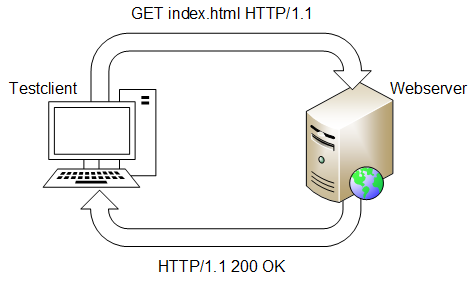
\includegraphics[scale=1]{figures/httpget.png}

\subsubsection{SSH}

\end{document}

